\section{浮点数}
\subsection{传统小数的二进制表示}在二进制中,小数点左侧每一位的权重为\(2^{i}\),右侧为\(\frac{1}{2^{i}}\)(位置计数法),一个二进制数\(b\)可以表示为\(b=\sum\limits_{i = -n}^{m}2^{i}\times b_{i}\)。例如:$5\frac{3}{4} = 101.11_{2}$
$2\frac{7}{8}= 010.111_{2}$
\begin{figure}[H]
    \centering
    \captionsetup{skip=4pt}
    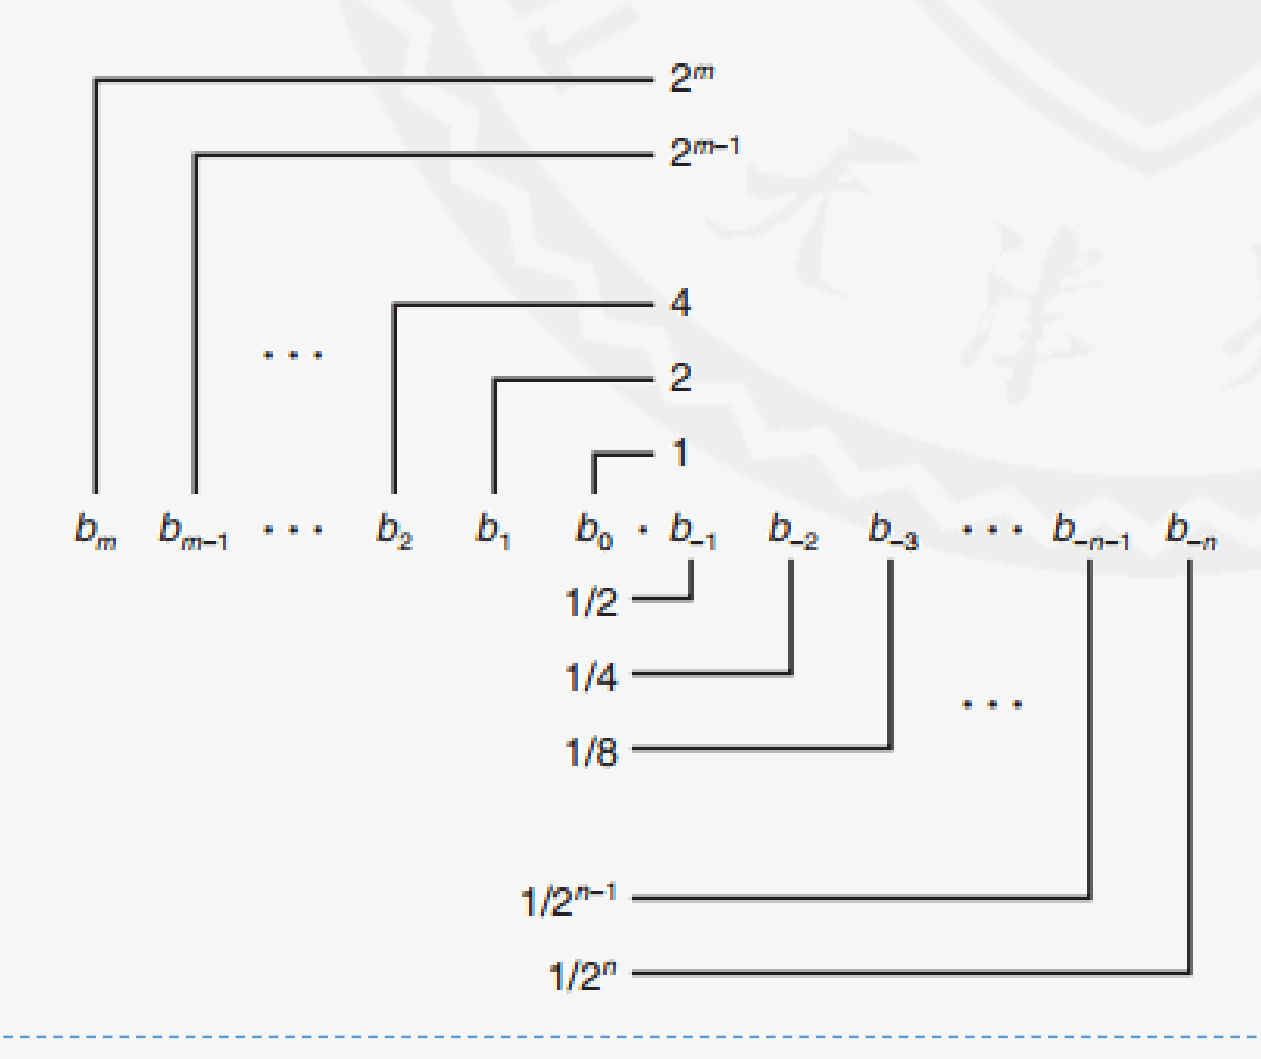
\includegraphics[width=6cm]{figures/1.png}
    \caption{小数的二进制表示}
\end{figure}


并且,除以2可通过逻辑右移实现,乘以2可通过左移实现。像\(0.11111\cdots_{2}\)这样的数字十分接近但小于1,可表示为\(1.0-\varepsilon\)。同时,并非所有有理数都能精确地用有限位二进制小数表示,例如\(\frac{1}{3}=0.0101010101[01]\cdots_{2}\),只能精确表示\(\frac{x}{2^{k}}\)这种形式的数字。

\subsection{IEEE浮点数的表示}
浮点数的表示形式为\((-1)^{s}\times M\times2^{E}\),其中:
\begin{itemize}
    \item 符号位\(s\)决定了数字的正负。
    \item 尾数\(M\)通常在\([1.0,2.0)\)或\([0.0,1.0)\)。
    \item 阶码\(E\)是浮点数的权重,为2的\(E\)次幂。
\end{itemize}
\begin{figure}[H]
    \centering
    \captionsetup{skip=4pt}
    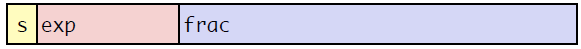
\includegraphics[width=10cm]{2.png}
    \caption{浮点数编码}
\end{figure}

编码方式为:最高位是符号位\(s\),\(\text{exp}\)编码后得到\(E\)(\(\text{exp}\neq E\)),\(\text{frac}\)编码后得到\(M\)(\(\text{frac}\neq M\))。

\subsubsection{几种精度的浮点数}

常见的浮点数精度有:
\begin{table}[h]
    \centering
    \begin{tabular}{|c|c|c|c|c|}
        \hline
        精度类型           & 总位数 & 符号位 & \(\text{exp}\)位数 & \(\text{frac}\)位数 \\
        \hline
        单精度            & 32位 & 1位  & 8位               & 23位               \\
        双精度            & 64位 & 1位  & 11位              & 52位               \\
        扩展精度(仅Intel支持) & 80位 & 1位  & 15位              & 63或64位            \\
        \hline
    \end{tabular}
    \caption{不同精度浮点数的位宽分布}
\end{table}

\subsubsection{规格化数}
当\(\text{exp}\neq000\cdots0\)且\(\text{exp}\neq111\cdots1\)时:
\begin{itemize}
    \item 尾数编码为包含一个隐式前置的1,即\(M = 1.x_1 x_2{\cdots}\),其中\(x_1x_2\cdots\)为\(\text{frac}\)域的各位的编码。
    \item 阶码为一个有偏置的指数,\(E=\text{Exp}-\text{Bias}\),\(\text{Exp}\)为\(\text{exp}\)域无符号数编码值,\(\text{bias}=2^{k - 1}-1\),\(k\)是\(\text{exp}\)的位宽。
    \item 例如,对于单精度浮点数,\(\text{bias}=127\)(\(\text{Exp}:1\cdots254\),\(E:-126\cdots127\));双精度浮点数,\(\text{bias}=1023\)(\(\text{Exp}:1\cdots2046\),\(E:-1022\cdots1023\))。隐式前置的整数1始终存在,因此在\(\text{frac}\)中不需要包含。
\end{itemize}
以\(\text{float }f = 15213.0\)为例:
\begin{align*}
    f=15213_{10}      & =1101101101101000000000_{2}           \\
                      & =1.1101101101101101_{2}\times2^{13}   \\
    \text{尾数 }\quad M & =1.\textbf{1101101101101101}_{2}      \\
    \text{frac}       & =\textbf{1101101101101} 000000000_{2} \\
    \text{阶码 }\quad E & =13,                                  \\
    \text{Bias}       & =2^{k-1}-1=127\quad(k=8),             \\
    \text{Exp}        & =140 = 10001100_{2}
\end{align*}
结果为\(0\quad10001100  \quad11011011011010000000000\)。

\subsubsection{非规格化数}
当\(\text{exp}=000\cdots0\)时:
\begin{itemize}
    \item 阶码\(E=-\text{Bias}+1\)(而不是\(E = 0-\text{Bias}\))。
    \item 尾数编码为包含一个隐式前置的0,即\(M = 0.x_1x_2\cdots\)。
    \item 当\(\text{exp}=000\cdots0\),且\(\text{frac}=000\cdots0\)时,表示0,要注意\(+0\)和\(-0\)的区别。
    \item 当\(\text{exp}=000\cdots0\),且\(\text{frac}\neq000\cdots0\)时,表示非常接近于0.0的数字,这些数字是等间距的。
\end{itemize}

\subsubsection{特殊值}
当\(\text{exp}=111\cdots1\)时:
\begin{itemize}
    \item 当\(\text{exp}=111\cdots1\)且\(\text{frac}=000\cdots0\)时,表示无穷\(\infty\),意味着运算出现了溢出,有正向溢出和负向溢出,例如\(1.0/0.0=-1.0/-0.0=+\infty\),\(1.0/-0.0=-\infty\)。
    \item 当\(\text{exp}=111\cdots1\)且\(\text{frac}\neq000\cdots0\)时,表示不是一个数字(NaN),表示数值无法确定,例如\(-1,\infty-\infty,\infty\times0\)。
\end{itemize}

\subsubsection{IEEE编码的特殊属性}
\begin{enumerate}
    \item 浮点数0和整数0编码相同,所有位都为0
    \item 几乎可以用无符号整数比较的方法实现浮点数的比较运算,但首先要比较符号位,同时要考虑\(-0 = 0\)和NaN的问题(NaN比其他值都大)
\end{enumerate}

\subsubsection{需要关注的数字}
不同类型的浮点数有一些特殊的数字:
\begin{table}[h]
    \centering
    \begin{tabular}{|c|c|c|c|c|c|}
        \hline
        描述      & \(\text{exp}\) & \(\text{frac}\) & 单精度值(十进制)                         & 双精度值(十进制)                          \\
        \hline
        零       & \(00\cdots00\) & \(0\cdots00\)   & 0.0                               & 0.0                                \\
        最小非规格化数 & \(00\cdots00\) & \(0\cdots01\)   & \(2^{-23}\times2^{-126}\)         & \(2^{-52}\times2^{-1022}\)         \\
        最大非规格化数 & \(00\cdots00\) & \(1\cdots11\)   & \((1-\varepsilon)\times2^{-126}\) & \((1-\varepsilon)\times2^{-1022}\) \\
        最小规格化数  & \(00\cdots01\) & \(0\cdots00\)   & \(1\times2^{-126}\)               & \(1\times2^{-1022}\)               \\
        一       & \(01\cdots11\) & \(0\cdots00\)   & 1.0                               & 1.0                                \\
        最大规格化数  & \(11\cdots10\) & \(1\cdots11\)   & \((2-\varepsilon)\times2^{127}\)  & \((2-\varepsilon)\times2^{1023}\)  \\
        \hline
    \end{tabular}
    \caption{不同精度浮点数的特殊值}
\end{table}

\subsubsection{举例:一个微型的浮点数编码系统}
以8位浮点数编码为例,最高位为符号位,接下来是4位\(\text{exp}\),偏置\(\text{Bias}\)为7,最后3位是\(\text{frac}\),与IEEE规范具有相同的形式,有规格化数、非规格化数,以及0、NaN和无穷的编码。
\begin{table}[h]
    \centering
    \begin{tabular}{|c|c|c|c|c|}
        \hline
        \(s\)  & \(\text{exp}\) & \(\text{frac}\) & \(E\)   & 值                                                     \\
        \hline
        0      & 0000           & 000             & -6      & 0                                                     \\
        0      & 0000           & 001             & -6      & \(\frac{1}{8}\times\frac{1}{64}=\frac{1}{512}\)(最接近0) \\
        \vdots & \vdots         & \vdots          & \vdots  & \vdots                                                \\
        0      & 1111           & 000             & \(n/a\) & inf                                                   \\
        \hline
    \end{tabular}
    \caption{8位浮点数编码示例}
\end{table}

\subsubsection{总结}
单精度浮点数可分为以下几类:
\begin{enumerate}
    \item 规格化数:\(\text{exp}\neq0000000\)且\(\text{exp}\neq11111111\)。
    \item 非规格化数:\(\text{exp}=00000000\),\(\text{frac}\neq0000000\)。
    \item 无穷:\(\text{exp}=11111111\),\(\text{frac}=00000000\)。
    \item NaN:\(\text{exp}=11111111\),\(\text{frac}\neq00000000\)。
\end{enumerate}




\subsection{几种舍入模式}
常见的舍入模式有:
\begin{enumerate}
    \item 向下舍入:舍入结果接近但不会大于实际结果。
    \item 向上舍入:舍入结果接近但不会小于实际结果。
    \item 向0舍入:舍入结果向0的方向靠近,如果为正数,舍入结果不大于实际结果;如果为负数,舍入结果不小于实际结果。
    \item 向偶数舍入:浮点数运算默认的舍入模式,其他的舍入模式都会统计偏差,一组正数的总和将始终被高估或低估。
\end{enumerate}
向偶数舍入适用于舍入至小数点后任何位置,当数字正好处在四舍五入的中间时,向最低位为偶数的方向舍入。例如:

\begin{table}[H]
    \captionsetup{skip=4pt}
    \centering
    \setlength{\arrayrulewidth}{1pt}
    \begin{tabular}{ccc}
        \hline
        \makebox[0.2\textwidth][c]{值} & \makebox[0.2\textwidth][c]{结果} & \makebox[0.4\textwidth][c]{说明} \\
        \noalign{\global\setlength{\arrayrulewidth}{0.5pt}}
        \hline
        1.2349999                     & 1.23                           & 比中间值小,四舍                       \\
        1.2350001                     & 1.24                           & 比中间值大,五入                       \\
        1.2350000                     & 1.24                           & 中间,向上舍入(偶数方向)                  \\
        1.2450000                     & 1.24                           & 中间,向下舍入(偶数方向)                  \\
        \noalign{\global\setlength{\arrayrulewidth}{1pt}}
        \hline
    \end{tabular}
    \caption{向偶数舍入示例}
\end{table}

在二进制数中,偶数方向意味着舍入后最后一位为0,中间意味着待舍入的部分为\(100\cdots_{2}\)。

\subsection{浮点数运算}
浮点数运算的基本思想是先计算出精确的值,然后将结果调整至目标的精度。如果阶码值过大,可能会导致溢出,可能会进行舍入以满足尾数的位宽。例如:
\begin{align*}
    x+^{f}y      & =\text{Round}(x + y)     \\
    x\times^{f}y & =\text{Round}(x\times y)
\end{align*}

\subsubsection{浮点数乘法}
对于浮点数\((-1)^{s_1}M_1 2^{E_1}\times(-1)^{s_2}M_2 2^{E_2}\):
\begin{itemize}
    \item 精确结果:\(M_1\times M_2\),阶码\(E = E_1 + E_2\),符号位\(s = s_1^{s_2}\)。
    \item 修正:如果\(M\geq2\),右移\(M\),并增大\(E\)的值;如果\(E\)超出范围,发生溢出;对\(M\)进行舍入以满足\(\text{frac}\)的位宽精度要求。在实际实现中,尾数相乘的细节较为繁琐。
\end{itemize}

\subsubsection{浮点数加法}
对于浮点数\((-1)^{s_1}M_1 2^{E_1}+(-1)^{s_2}M_2 2^{E_2}\)(假设\(E_1>E_2\)):
\begin{itemize}
    \item 精确结果:\((-1)^{s}M_2^{E}\),其中符号位\(s\)和尾数\(M\)是有符号数对齐后相加的结果,阶码\(E = E_2\)。
    \item 修正:如果\(M\geq2\),右移\(M\),并增大\(E\)的值;如果\(M<1\),左移\(M\) \(k\)位,然后\(E\)减去\(k\);如果\(E\)超出范围,发生溢出;对\(M\)进行舍入以满足\(\text{frac}\)的位宽精度要求。
\end{itemize}

\subsection{C语言中的浮点数}
C语言标准确保支持两种精度的浮点数,即float(单精度)和double(双精度)。在进行类型转换时:
\begin{itemize}
    \item double/float转int:截断尾数部分,向0舍入。标准中未定义越界和NaN的情况,通常设置为\(T_{Min}\)和\(T_{Max}\)。
    \item int转double:只要int的位宽小于等于53位,就能精确转换。
    \item int转float:会根据舍入模式进行舍入。
\end{itemize}

以下是一些C语言中浮点数操作的示例(假设d和f分别是float和double且不是NaN和无穷):

\begin{table}[H]
    \captionsetup{skip=4pt}
    \centering
    \setlength{\arrayrulewidth}{1pt}
    \begin{tabular}{cc}
        \hline
        \makebox[0.4\textwidth][c]{表达式}                      & \makebox[0.4\textwidth][c]{结果} \\
        \noalign{\global\setlength{\arrayrulewidth}{0.5pt}}
        \hline
        \lstinline[style=cstyle]{x == (int)(float) x}        & 否:有效数字为24位                     \\
        \lstinline[style=cstyle]{x == (int)(double) x}       & 是:有效数字为53位                     \\
        \lstinline[style=cstyle]{f == (float)(double) f}     & 是:提高精度                         \\
        \lstinline[style=cstyle]{d == ( float ) d}           & 否:丢失精度                         \\
        \lstinline[style=cstyle]{f == -(-f)}                 & 是:仅改变符号位                       \\
        \lstinline[style=cstyle]{2/3 == 2/3.0}               & 否:\(2/3 == 0\)                 \\
        \lstinline[style=cstyle]{if(d < 0.0)  ((d*2) < 0.0)} & 是                              \\
        \lstinline[style=cstyle]{d * d >= 0.0}               & 是                              \\
        \lstinline[style=cstyle]{(d + f) - d == f}           & 否:不满足结合律                       \\
        \noalign{\global\setlength{\arrayrulewidth}{1pt}}
        \hline
    \end{tabular}
    \caption{C语言中浮点数操作示例结果}
\end{table}

在浮点数运算中,存在精度和准确度的问题。例如\(0.1 + 0.1 + 0.1 + 0.1 + 0.1 + 0.1 + 0.1 + 0.1 + 0.1+ 0.1 \neq1\),但\(0.2+0.2+0.2+0.2+0.2=1\)。在使用浮点数进行比较时,如\lstinline[style=cstyle]{if (d1 - d2 == 0)},需要谨慎处理,因为浮点数的精度限制可能导致结果不准确。在进行浮点数运算时,要充分考虑精度损失对计算结果的影响。
